\documentclass[a4paper,12pt]{extarticle}
\usepackage[utf8x]{inputenc}
\usepackage[T1,T2A]{fontenc}
\usepackage[russian]{babel}
\usepackage[hidelinks]{hyperref}
\usepackage{indentfirst}
\usepackage{listings}
\usepackage{color}
\usepackage{here}
\usepackage{array}
\usepackage{multirow}
\usepackage{graphicx}
\usepackage{subcaption} 
\usepackage{mathtools}
\usepackage{listings}

\usepackage{caption}
\renewcommand{\lstlistingname}{Программа} % заголовок листингов кода

\bibliographystyle{ugost2008ls}

\usepackage{listings}
\lstset{ %
extendedchars=\true,
keepspaces=true,
language=C,						% choose the language of the code
basicstyle=\footnotesize,		% the size of the fonts that are used for the code
numbers=left,					% where to put the line-numbers
numberstyle=\footnotesize,		% the size of the fonts that are used for the line-numbers
stepnumber=1,					% the step between two line-numbers. If it is 1 each line will be numbered
numbersep=5pt,					% how far the line-numbers are from the code
backgroundcolor=\color{white},	% choose the background color. You must add \usepackage{color}
showspaces=false				% show spaces adding particular underscores
showstringspaces=false,			% underline spaces within strings
showtabs=false,					% show tabs within strings adding particular underscores
frame=single,           		% adds a frame around the code
tabsize=2,						% sets default tabsize to 2 spaces
captionpos=t,					% sets the caption-position to top
breaklines=true,				% sets automatic line breaking
breakatwhitespace=false,		% sets if automatic breaks should only happen at whitespace
escapeinside={\%*}{*)},			% if you want to add a comment within your code
postbreak=\raisebox{0ex}[0ex][0ex]{\ensuremath{\color{red}\hookrightarrow\space}},
texcl=true,
inputpath=listings,                     % директория с листингами
}

\usepackage[left=2cm,right=2cm,
top=2cm,bottom=2cm,bindingoffset=0cm]{geometry}

%% Нумерация картинок по секциям
\usepackage{chngcntr}
\counterwithin{figure}{section}
\counterwithin{table}{section}

%%Точки нумерации заголовков
\usepackage{titlesec}
\titlelabel{\thetitle.\quad}
\usepackage[dotinlabels]{titletoc}

%% Оформления подписи рисунка
\addto\captionsrussian{\renewcommand{\figurename}{Рисунок}}
\captionsetup[figure]{labelsep = period}

%% Подпись таблицы
%\DeclareCaptionFormat{hfillstart}{\hfill#1#2#3\par}
%\captionsetup[table]{format=hfillstart,labelsep=newline,justification=centering,skip=-10pt,textfont=bf}

%% Путь к каталогу с рисунками
\graphicspath{{fig/}}

%% Внесение titlepage в учёт счётчика страниц
\makeatletter
\renewenvironment{titlepage} {
 \thispagestyle{empty}
}
\makeatother

\DeclarePairedDelimiter\abs{\lvert}{\rvert}%
\DeclarePairedDelimiter\norm{\lVert}{\rVert}%

\usepackage{amsmath}

\lstset{language=Java} 

\begin{document}	% начало документа

% Титульная страница
\begin{titlepage}	% начало титульной страницы

	\begin{center}		% выравнивание по центру

		\large Санкт-Петербургский политехнический университет Петра Великого\\
		\large Институт прикладной математики и механики \\
		\large Высшая школа прикладной математики и вычислительно физики \\[6cm]
		% название института, затем отступ 6см
		
		\huge Вычислительные комплексы\\[0.5cm] % название работы, затем отступ 0,5см
		\large \textbf{Курсовой проект}\\[5.1cm]

	\end{center}


	\begin{flushright} % выравнивание по правому краю
		\begin{minipage}{0.25\textwidth} % врезка в половину ширины текста
			\begin{flushleft} % выровнять её содержимое по левому краю

				\large\textbf{Работу выполнил:}\\
				\large Колесник Виктор\\
				\large {Группа:} 3630102/70201\\
				
				\large \textbf{Преподаватель:}\\
				\large к.ф.-м.н., доцент\\
				\large Баженов Александр Николаевич

			\end{flushleft}
		\end{minipage}
	\end{flushright}
	
	\vfill % заполнить всё доступное ниже пространство

	\begin{center}
	\large Санкт-Петербург\\
	\large \the\year % вывести дату
	\end{center} % закончить выравнивание по центру

\end{titlepage} % конец титульной страницы

\vfill % заполнить всё доступное ниже пространство


% Содержание
\renewcommand\contentsname{\centerline{Содержание}}
\tableofcontents
\newpage

\listoffigures
\newpage


\section{Постановка задачи}

Требуется решить недоопределённую интервальную систему линейных алгебраических уравнений (ИСЛАУ) с матрицей 3x2 и переопределённую ИСЛАУ с матрицей 2x3. Используемые матрицы должны совпадать с точностью до транспонирования. \\
Найти допусковое множество решений, оценку вариабельности решения ive. \\
Для случая 3х2 построить график $\text{Tol}(x_1, x_2)$. \\
Для случая 2x3 проанализировать решение. \\
Построить 3-мерный образ допускового множества или его проекции на плоскости $(x_i O x_j)$.



\section{Теория}

\begin{itemize}

	\item Распознающий функционал для исследования разрешимости ИСЛАУ:
		\begin{equation}
			\text{Tol}(x)=\min_{1 \leq i \leq n} (\text{rad} b_i - |\text{mid} b_i - \sum_{j=1}^{m}a_{ij}x_j|)
		\end{equation}
	
	\item Мера вариабельности:
		\begin{equation}
			\text{ive}(\textbf{A}, \textbf{b})= \sqrt{n} (\min_{A \in \textbf{A}} \text{cond} A) * ||\arg \max \text{Tol} || * \frac{\max \text{Tol}}{||b||}
		\end{equation}
	
	\item Расчет бруса:
		\begin{equation}
			\tilde{x} = [ \arg \max \text{Tol} - \text{ive}, \arg \max \text{Tol} + \text{ive} ]
		\end{equation}

\end{itemize}



\section{Задача}

\subsection{Недоопределённая ИСЛАУ}
Возьмем матрицу $A$ следующего вида:
\begin{equation}
	A =
	\begin{pmatrix}
		4 & 3 & 5 \\
		1 & 7 & 6
	\end{pmatrix}
\end{equation}
Пусть решение СЛАУ имеет вид:
\begin{equation}
	x_0=
	\begin{pmatrix}
		1 & 1 & -1
	\end{pmatrix}^T
\end{equation}
Тогда вектор $b$ равен:
\begin{equation}
	A*x_0=b=
	\begin{pmatrix}
		2 & 2
	\end{pmatrix}^T
\end{equation}
Зададим радиусы для матрицы $\textbf{A}$ и вектора $\textbf{b}$:
\begin{equation}
	\text{rad} \textbf{A}=
	\begin{pmatrix}
		1 & 2 & 3 \\
		2 & 1 & 2
	\end{pmatrix}
\end{equation}
\begin{equation}
	\text{rad} \textbf{b}=
	\begin{pmatrix}
		1 & 2
	\end{pmatrix}^T
\end{equation}
Получим следующую недоопределённую интервальную СЛАУ:
\begin{equation}
	\textbf{A}=
	\begin{pmatrix}
		[3,5] & [1,5] & [2,8] \\
		[-1,3] & [6,8] & [4,8]
	\end{pmatrix}
\end{equation}
\begin{equation}
	\textbf{b}=
	\begin{pmatrix}
		[1,3] & [0,4]
	\end{pmatrix}^T
\end{equation}


\subsection{Переопределённая ИСЛАУ}
Из предыдущего пункта задана следующая матрица $A$:
\begin{equation}
	A =
	\begin{pmatrix}
		4 & 1 \\
		3 & 7 \\
		5 & 6
	\end{pmatrix}
\end{equation}
Пусть вектор-решение $x_0$ имеет вид:
\begin{equation}
	x_0=
	\begin{pmatrix}
		1 & -1
	\end{pmatrix}^T
\end{equation}
Тогда вектор $b$ равен:
\begin{equation}
	A*x_0=b=
	\begin{pmatrix}
		3 & -4 & -1
	\end{pmatrix}^T
\end{equation}
Зададим радиус для вектора $\textbf{b}$:
\begin{equation}
	\text{rad} \textbf{b}=
	\begin{pmatrix}
		3 & 5 & 6
	\end{pmatrix}^T
\end{equation}
Получим следующую переопределённую интервальную СЛАУ:
\begin{equation}
	\textbf{A} =
	\begin{pmatrix}
		[3,5] & [-1,3] \\
		[1,5] & [6,8] \\
		[2,8] & [4,8]
	\end{pmatrix}
\end{equation}
\begin{equation}
	\textbf{b}=
	\begin{pmatrix}
		[0,6] & [-9,1] & [-7, 5]
	\end{pmatrix}^T
\end{equation}



\section{Результаты}

\subsection{Недоопределённая ИСЛАУ}
Решим задачу с помощью функции $\text{tolsolvty}$. Получим максимум распознающего функционала $\text{Tol}$ и значение аргумента, в котором максимум достигался:
\begin{equation}
	\max \text{Tol} = 0.3437
\end{equation}
\begin{equation}
	\arg \max \text{Tol}=
	\begin{pmatrix}
		0.406 \\
		0.125 \\
		1.377 * 10^{-7}
	\end{pmatrix}
\end{equation}

\subsubsection{Оценка меры вариабельности ive}
Минимальное число обусловленности матрицы $A$ равно:
\begin{equation}
	\min \text{cond} \textbf{A} = 2.2427
\end{equation}
Оценка меры вариабельности равна:
\begin{equation}
	\text{ive}(\textbf{A}, \textbf{b}) = 0.1638
\end{equation}
Брус оценки имеет вид:
\begin{equation}
	\tilde{x} =
	\begin{pmatrix}
	    [0.2424, 0.5701] \\
		[-0.0388, 0.2888] \\
		[-0.1638, 0.1638]
	\end{pmatrix}
\end{equation}

\subsubsection{Допусковое множество решений}
Построим график допускового множества решений с помощью функции EqnTol3D. Добавим брус оценки и вектор, в котором достигается максимум распознающего функционала. Допусковое множество представлено зеленой областью, вектор - фиолетовой звездой, брус - черными линями, представляющими его рёбра. \\
\begin{figure}[h]
	\centering
	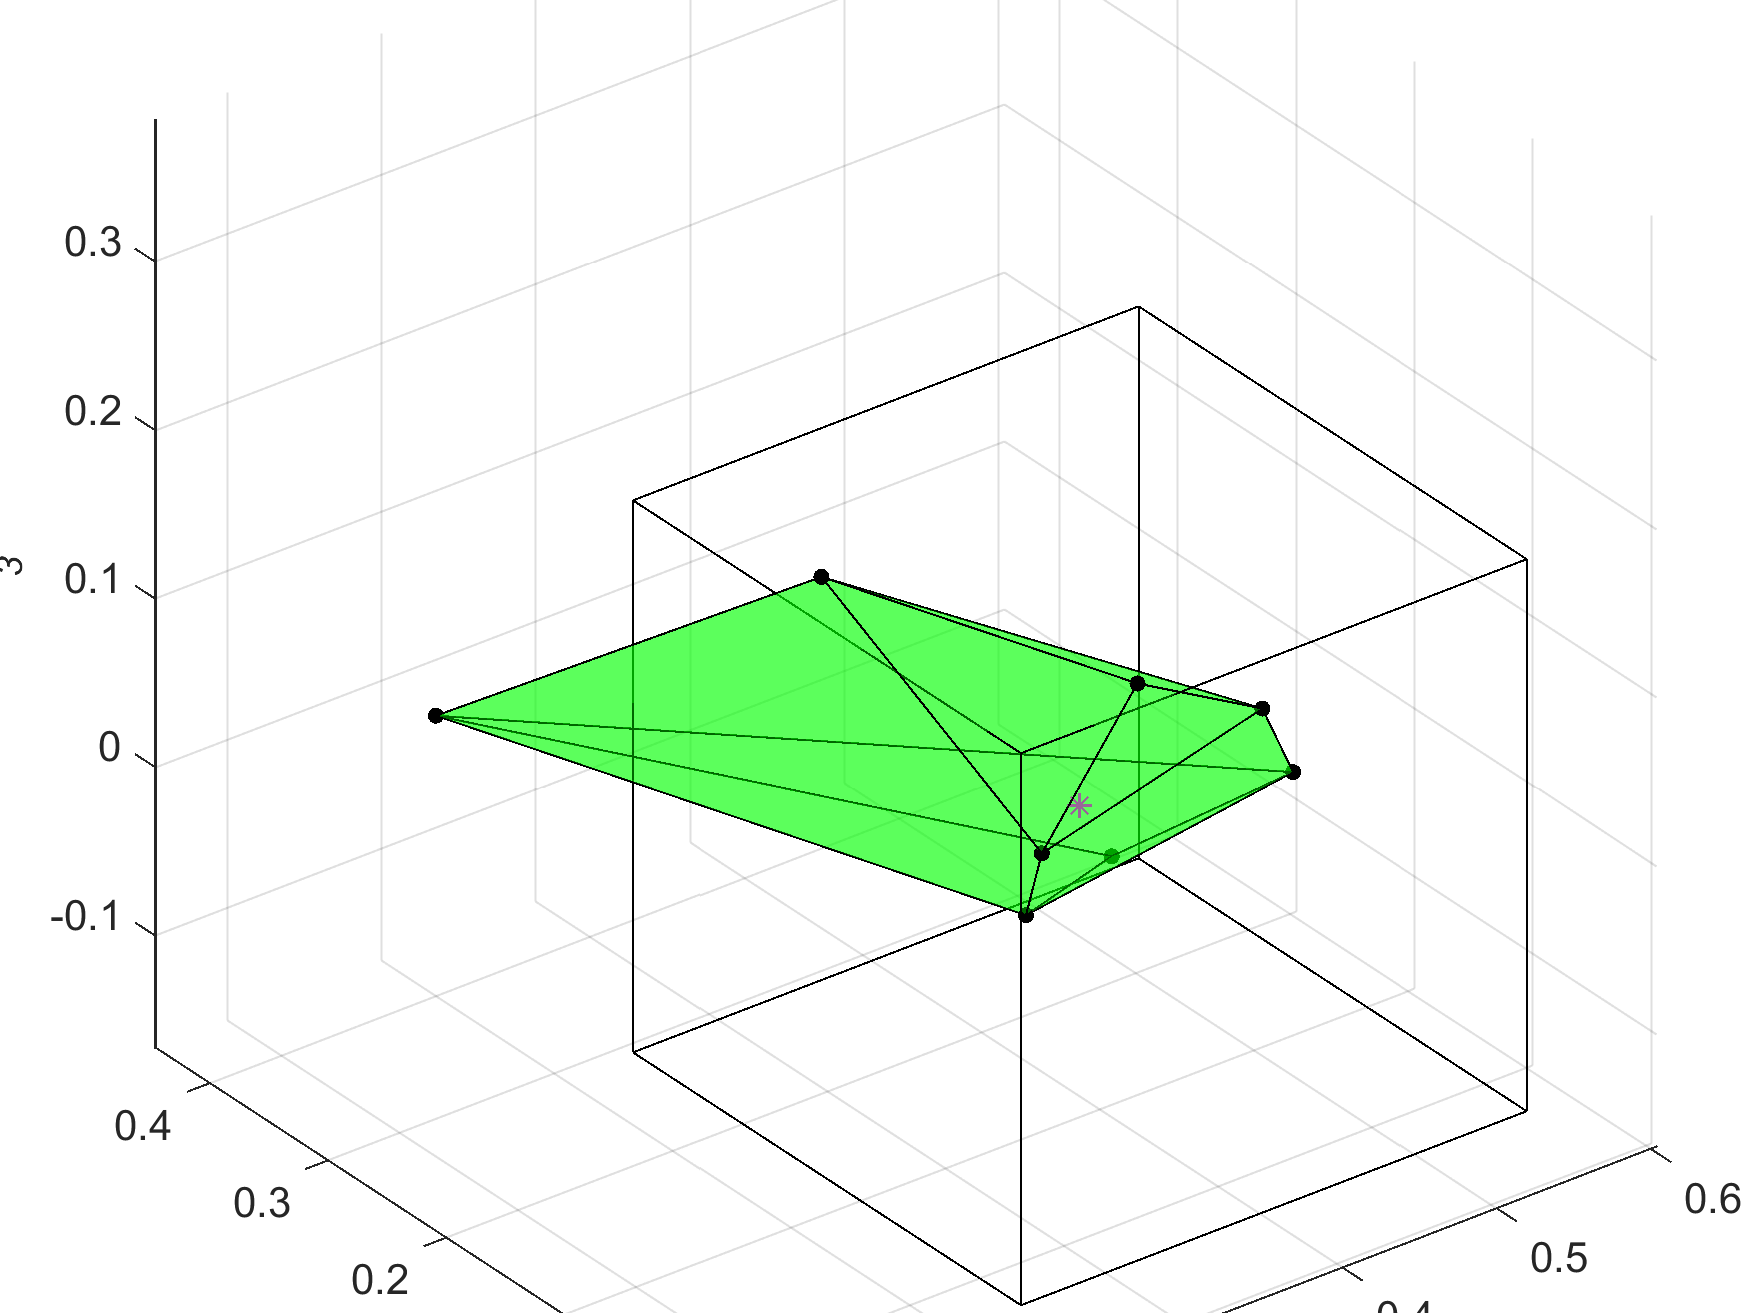
\includegraphics[width=0.75\textwidth]{ISLAU Solution2x3.png}
	\caption{Допусковое множество решений недопределённой ИСЛАУ}
\end{figure} \\
Так как 3 координата вектора $\arg \max \text{Tol}$ практически равна 0, можно рассмотреть брус 2D-проекции на плоскость $x_1 O x_2$. \\
\newpage
\begin{figure}[h]
	\centering
	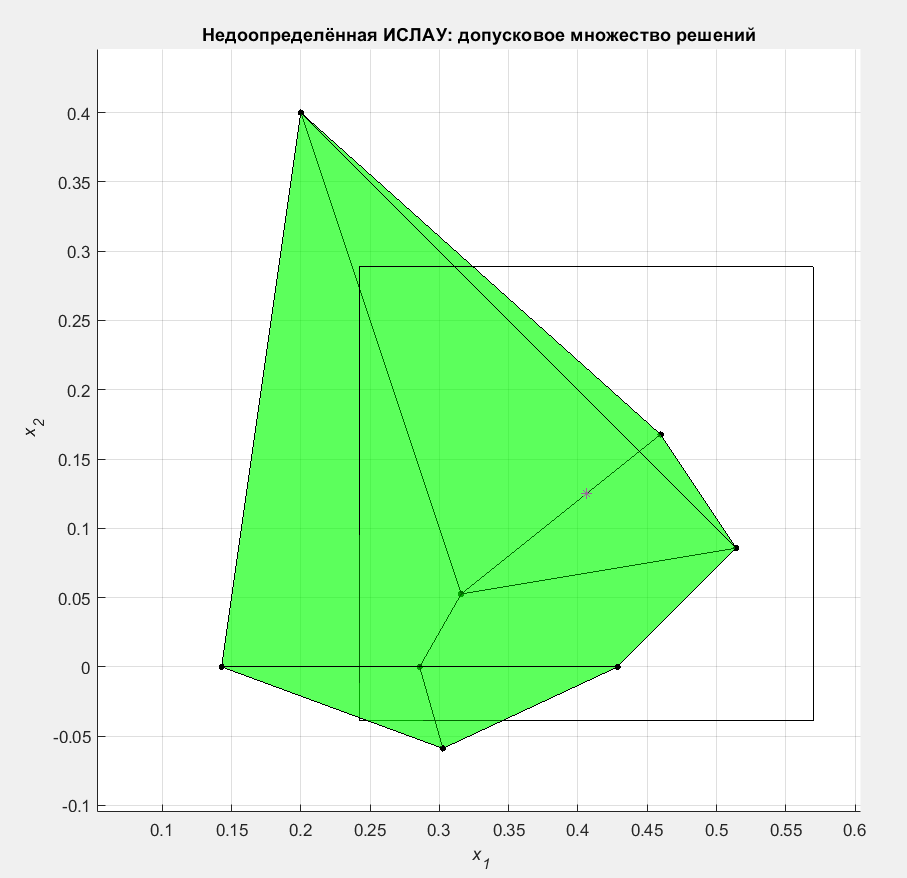
\includegraphics[width=0.75\textwidth]{islau2x3.png}
	\caption{Допусковое множество решений недопределённой ИСЛАУ. Проекция на $x_1 O x_2$}
\end{figure}
Стоит отметить, что брус не покрывает все допусковое множество решений. \\

\subsubsection{Анализ решения}

Можно заметить, что полученное решение ИСЛАУ $\arg \max \text{Tol}$ сильно отличается от $x_0$: \\
\begin{equation}
	\arg \max \text{Tol}=
	\begin{pmatrix}
		0.406 \\
		0.125 \\
		1.377 * 10^{-7}
	\end{pmatrix} \neq x_0 = 
	\begin{pmatrix}
		1 \\
		1 \\
		-1
	\end{pmatrix}
\end{equation} \\
Тем не менее, $\arg \max \text{Tol}$ удовлетворяет границам правой части:
\begin{equation}
	\textbf{A} * \arg \max \text{Tol} = 
		\begin{pmatrix}
			[1.3429, 2.6551]  \\
			[0.3439, 2.2181] 
		\end{pmatrix}
	\subseteq \textbf{b}
\end{equation} \\
Такой результат - проявление неоднозначности решения обратной задачи. Кроме того, для СЛАУ, которая в неинтервальной постановке имела бы бесконечное множество решений, методами интервального анализа было получено конечное множество решений.



\subsection{Переопределённая ИСЛАУ}
Решим задачу с помощью функции $\text{tolsolvty}$. Получим максимум распознающего функционала $\text{Tol}$ и значение аргумента, в котором максимум достигался:
\begin{equation}
	\max \text{Tol} = 0.6279
\end{equation}
\begin{equation}
	\arg \max \text{Tol}=
	\begin{pmatrix}
		0.8837 \\
		-0.6744
	\end{pmatrix}
\end{equation}

\subsubsection{Оценка меры вариабельности ive}
Минимальное число обусловленности матрицы $A$ от транспонирования не меняется и равно:
\begin{equation}
	\min \text{cond} \textbf{A} = 2.2427
\end{equation}
Оценка меры вариабельности равна:
\begin{equation}
	\text{ive}(\textbf{A}, \textbf{b}) = 0.4342
\end{equation}
Брус оценки имеет вид:
\begin{equation}
	\tilde{x} =
	\begin{pmatrix}
		[0.4495, 1.3179] \\
		[-1.1086, -0.2402]
	\end{pmatrix}
\end{equation}

\subsubsection{Допусковое множество решений}
Построим график допускового множества решений с помощью функции EqnTol2D. Добавим брус оценки и вектор, в котором достигается максимум распознающего функционала. Допусковое множество представлено зеленой областью, вектор - красной квадратной точкой, брус - черным квадратом. \\
\newpage
\begin{figure}[h]
	\centering
	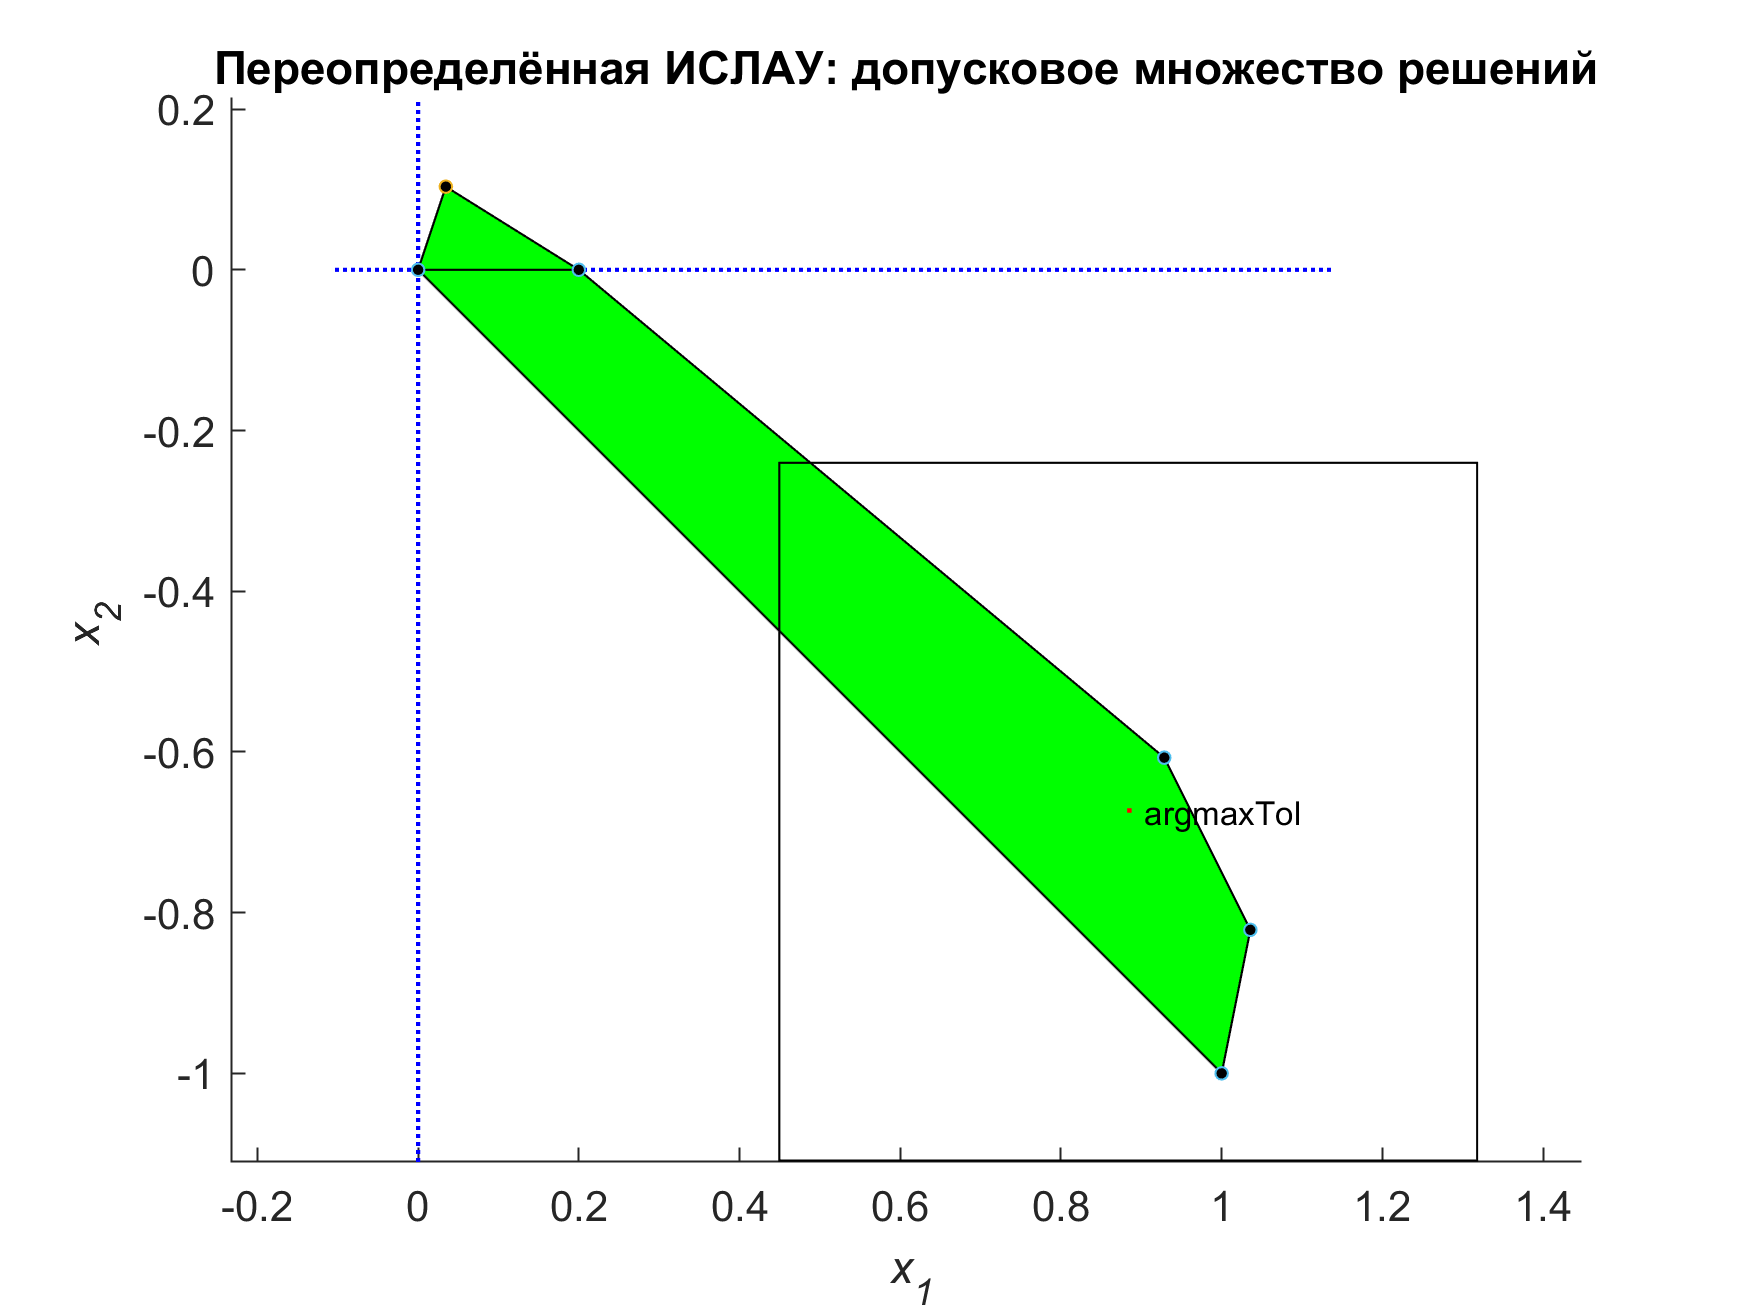
\includegraphics[width=0.75\textwidth]{islau solution3x2.png}
	\caption{Допусковое множество решений переопределённой ИСЛАУ}
\end{figure}

\subsubsection{График распознающего функционала}
Построим график распознающего функционала $\text{Tol}(x_1, x_2)$. Красным кружком обозначена точка, в которой функционал достигает максимальное значение. \\
\newpage
\begin{figure}[h]
	\centering
	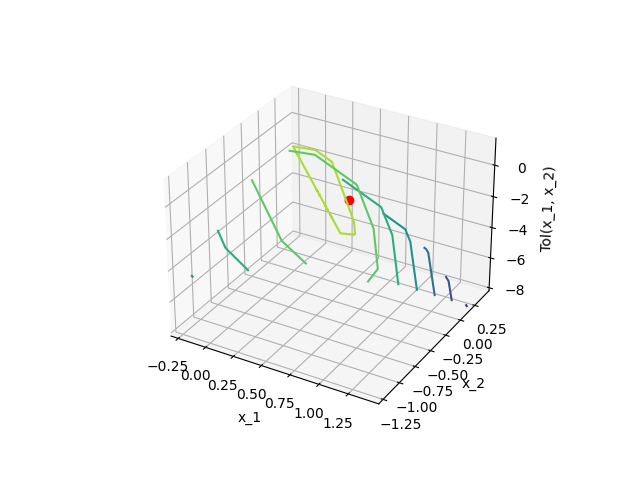
\includegraphics[width=0.75\textwidth]{Tol(x_1, x_2).png}
	\caption{Распознающий функционал}
\end{figure}



\section{Приложение}
Код программы на Python и MATLAB лежит в данном репозитории: \\
\url{https://github.com/PinkOink/Interval_Analysis/tree/main/lab3}{}

Реализация функции tolsolvty на Python: \\
\url{https://github.com/MaximSmolskiy/tolsolvty}{}

Пакет IntLinInc2D: \\
\url{http://interval.ict.nsc.ru/Programing/MCodes/IntLinInc2D.zip}{}

Пакет IntLinInc3D: \\
\url{http://interval.ict.nsc.ru/Programing/MCodes/IntLinInc3D.zip}{}


\end{document}